\documentclass{cup-ino}
\usepackage[utf8]{inputenc}
\usepackage{longtable}
\usepackage{blindtext,alltt}
\usepackage{times}
\usepackage{fancyhdr,graphicx,amsmath,amssymb}
% \usepackage{algorithm} 
% \usepackage{algorithmic}
\usepackage[ruled,vlined]{algorithm2e}
% \usepackage[ruled,linesnumbered]{algorithm2e}
\include{pythonlisting}

\usepackage{graphicx}
\graphicspath{ {.} }



%% Full title
\title{\item Tunable Survivability on Off-chain network}

%% Shorter title, for use in page header
\runningtitle{Tunable Survivability on Off-chain network}
\author{Hagay Michaeli and Uri Gadot}

%% The .bib file containing reference entires, for use with biblatex. CUP-INO loads the biblatex-chicago package with customisations for INO.
\addbibresource{refs.bib}

\begin{document}

\maketitle

%\begin{abstract}
%TODO
%\end{abstract}

\section{Intro}
As block-chain usage increased in the last decade, its scalability restrictions are more relevant then ever. The fact that each transaction needs to be written inside a block, which is added to the chain on average time of 10 minutes, does not allow Block-chain based currency users to conduct quick transactions. Off-chain was introduced lately in order to allow block-chain users, to conduct those transactions with low latency waiting time.
The basic concept is creating a paying channel between 2 users, which is backed up with some currency on the original block-chain network. These deposits dictate the channel capacity, thus guarantee that no user would have unsettled debts.
The created channels can be used as an external network:
Users can transfer money on a path of several different existing channels, thus creating a new network, an "Off-chain" network.\\
Since creating a new channel requires an "On-Chain" transaction, it is expensive and has low-latency. Therefore, we rather create an "Off-chain" topology that requires as least "On-chain" deposits as possible, while allowing as many "Off-chain" transactions as possible. In particular, we are interested in generating a topology that suffices the transaction requirements in a certain probability, which will be denoted as the network survivability.  \\
Our work focuses on those two restrictions in-order to give a good cost-effective solution.\\
Previous work was done in finding optimal off-chain in terms of minimal deposits and transaction fees. \footcite{9352899}
The idea of graph survivability was initially presented as a constraint for routing trees. \footcite{7163640}

\section{Assumptions and Modelling}
In order to model the problem easily, we would like to make several assumption:\\
\begin{enumerate}
    \item Once a route path was chosen over the "Off-chain" network, all transaction between the users are done on the same path. if there are no sufficient deposit left, the transaction fails.
    \item We are considering 0 fees with regards to the routing path chosen, thus making the deposit amount the only cost metric involved in our algorithm.
    \item We are assuming that the transaction demands are periodical and occur randomly with a given distribution over a specific time interval. 
\end{enumerate}
\\\\
In addition, lets define the following:\\
The number of users on the "Off-chain" network would be denoted as $N$.\\
Off-chain payments demands between users $v$ and $u$ would be denoted as $d(v,u)$. The amount of payment that user $v$ wants to transfer to user $u$ on a given time period has Gaussian distribution with mean $\mu$ and variance $\sigma ^2$.  (e.g. if between users $v_1$ and $v_2$ the distribution is: $P_{v_1,v_2} \sim (0,0)$ then the users are not transferring currency, while on the other hand if the distribution is: $P_{v_1,v_2} \sim (1,0)$, then user $v_1$ is always transferring 1 currency to use $v_2$).\\
Lets denote an anti-symmetric matrix $M$ that represent the payments mean values between each 2 users of the "Off-chain".\\
We would also denote symmetric matrix $S$ that represent the payments variance values between each 2 users of the "Off-chain".\\
Because each user can never pay for himself we get: $\forall i<N$, $M[i,i] = S[i,i] = 0$.\\ \\
Using Gaussian distribution as payments demand over time can be beneficial for several reasons:
\begin{enumerate}
    \item Gaussian distribution over time can be easily modelled with given data
    \item Calculating the probability of a given payment to be above / under a certain value is done more easily with Gaussian distribution
    \item Summing several independent Gaussian variables is also easy to calculate.\\
\end{enumerate}
\\
* Example of the intuition behind this usage appear on Appendix 1.
\\\\
Given an "Off-chain" channel between users $v$ and $u$, we can denote this channel: $c(u,v)$. We can also denote the amount of deposit for each user as $C_v$ and $C_u$.
Finally, lets denote the matrix $C$ as the deposit for each user on all of it's "Off-chain" channels.\\
\\
As we mentioned before, the demand between user $v$ and user $u$ can have several different routes on the "Off-chain" network. Let's denote a "function"
$H:D \rightarrow C$ \\
For a given demand $d(u,v)$ the value of the function over this demand, is the channels its uses on it's route over the "Off-chain" network.
\begin{center}
$H(d)=\{c \in C | d $ uses payment channel $c\}$\\
\end{center}
In addition we can denote $H^{-1}:C \rightarrow D$ where for a given payment channel $c$ the function maps all the demands using this channel.
\begin{center}
$H^{-1}(c)=\{d \in D | d$ uses payment channel $c\}$.\\
\end{center}
\\
We defined the survivability of a channel as the probability of the accumulative demand over this channel to be lower than its deposit:
\begin{center}
    $S(c_{u,v}) = P_{success}(c_{u,v}) = P(-C_{u,v} \leq H^{-1}(c_{u,v}) \leq C_{v,u}) = \\
    P(-C_{u,v} \leq \Sigma_{d \in H^{-1}(c_{u,v})} d \leq C_{v,u}) = \\ 
    P(\Sigma_{d \in H^{-1}(c_{u,v})} d \leq C_{v,u}) - P(\Sigma_{d \in H^{-1}(c_{u,v})} d \leq -C_{u,v})$
\end{center}
Because all of the demands are Gaussian variables then:
\begin{center}
    $\Sigma_{d_{x,y} \in H^{-1}(c_{u,v})} d_{x,y} \sim N(\Sigma_{d_{x,y} \in H^{-1}(c_{u,v})} M[x,y], \Sigma_{d_{x,y} \in H^{-1}(c_{u,v})} S[x,y])$
\end{center}
\\
Now we can continue and define the survivability of the entire Graph as the average of survivability of every channel on the graph:
\begin{center}
    $S(G) = \frac{\Sigma_{c \in G} S(c)}{\Sigma_{c \in G}}$
\end{center}
\\
* Adding different weights to every channel can allow us to define importance of one channel against another thus creating weighted average:
\begin{center}
    $S(G) = \frac{\Sigma_{c \in G} w(c) \times S(c)}{\Sigma_{c \in G} w(c)}$
\end{center}
\\
For simplicity we would assume that the weights of each channel are equal: $w(c) = \frac{1}{N}$
\\\\
Because the survivability of each channel is a Probability the following always holds: $0 \leq S_0 \leq 1$\\
This allow us to \textbf{tune} the survivability level of the transactions over the graph, for example: lets set the desired survivability to $S_0 = 0.9$ thus by definition we want the following to hold:
\begin{center}
$S(G) \geq S_0$

$\frac{\Sigma_{c \in G} w(c) \times S(c)}{\Sigma_{c \in G} w(c)} \geq S_0$
\end{center}

Again, for simplicity we can demand a more strict condition, but easier to enforce:
\begin{center}
$\forall c \in G: S(c) \geq S_0$

$\implies S(G) = \frac{\Sigma_{c \in G} w(c) \times S(c)}{\Sigma_{c \in G} w(c)} \geq \frac{\Sigma_{c \in G} w(c) \times S_0}{\Sigma_{c \in G} w(c)} \geq S_0$
\end{center}
\\
Using this assumption we can define an algorithm to assure a certain amount of survivability  while trying to minimize the entire capacity of the graph:

\begin{center}
    $\min(C(G'))$ 

    s.t. $S(G') \geq S_0$
\end{center}
where:\\
$G'=(V,E) :$\\
$V = $ all Off-chain users.\\
$E = \{c | c \in G'\}$\\
$C(G) = \Sigma_{c \in G} C$\\
\\



\begin{algorithm}[H]

\SetAlgoLined
\KwIn{\\$D = Sorted\ Demands\ list;\\
    S_0 = Survivability;$ }
\KwOut{$G = Off-Chain Network$}

 \State $G = (V, \emptyset)$;\\
 \For{$d = (s, t, \mu, \sigma)$ in $D$}{
 \State Find all paths from $s$ to $t$;\\
 \For{ path from $s$ to $t$}{
 \State calculate required additional deposit to maintain $S_0$;\\
 }\EndFor
 \State calculate required deposit on direct path;\\
 \State choose minimal path;\\
 \State update $G$ deposits;\\
 }\EndFor             
 \caption{Create Off-Chain topology and required deposits}

\end{algorithm}

\\
\\
\\

\begin{algorithm}[H]
\SetAlgoLined
\KwIn{\\$P = Path\ from\ s\ to\ i;\\
        d = new\ demand\ to\ be\ added;\\
        S_0 = Survivability;$}
\KwOut{$A = additional\ deposit\ for: \forall c\ in\ P$}

 \For{$c\ in\ P, c \in G$}{
 save previous capacity on this channel: $old\_C = C$\\
 add $d$ to $H^{-1}(c)$ and calculate optimization problem** - $new\_C = optimize(c, S_0)$\\
 Calculate additional deposits in order to hold the desired survivability - $A = max(0, 2 \times (new\_C - old\_C))$*\\
 remove $d$ from $H^{-1}(c)$ and return $A$.
 
 }\EndFor             
 \caption{Calculate additional deposit to maintain $S_0$}
\end{algorithm}
\\
* $A$ is defined as $max(0, addition)$ in order to avoid minimum additions, for more tighter boundary over the total capacity we can add negative additions to the algorithm.\\
** The optimization problem is defined as follow:\\

\paragraph{Optimization Problem:}
We would like to minimize the deposits (capacity of the edges), subject to survivability constraint:
\begin{center}
$min \ \ x$

$ s.t \ \ \  \Phi(\frac{x -\mu}{\sigma}) - \Phi(\frac{-x -\mu}{\sigma}) \geq S_0 $
\end{center}
\\
where:\\
$x$ is the deposits on the edges - \textbf{for simplicity we assume same-size deposit on both edges.}\\
The total demand over the given channel ($c_{u,v}$) is:
\begin{center}
$\mathfrak{D}_{u,v} \sim N(\mu, \sigma) $ \\
\end{center}
 $\mathfrak{D}_{u,v} = \Sigma_{d_{x,y} \in H^{-1}(c_{u,v})} d_{x,y}$ \\
 $\mu = \Sigma_{d_{x,y} \in H^{-1}(c_{u,v})} M[x,y] \\$
 $\sigma = \Sigma_{d_{x,y} \in H^{-1}(c_{u,v})} S[x,y] \\$


This is a convex problem, so the solution for the deposits should satisfy
\begin{center}
$\Phi(\frac{x -\mu}{\sigma}) - \Phi(\frac{-x -\mu}{\sigma}) = S_0 $\\
\end{center}
\\
We used numerical algorithm to solve this equation, as there is no closed form solution to this equation.\\
by defining: $F(x) = \Phi(\frac{x -\mu}{\sigma}) - \Phi(\frac{-x -\mu}{\sigma}) - S_0$\\
and finding the roots $x_i$ that holds: $F(x_i) = 0$, we can get the minimum needed deposit in order to hold the survivability conditions.\\\\\\







\paragraph{Example:}
Assume 3 clients with demands:
\begin{center}
 \begin{tabular}{||c c c c||} 
 \hline
 Source & Target & \mu & \sigma \\ [0.5ex] 
 \hline\hline
 0& 1& 10& 1 \\
 \hline
 0& 2& -10& 1 \\
 \hline
 2& 1& -2& 0.5 \\
 \hline
\end{tabular}
\end{center}
the required survivability is $S_0 = 0.9$
\\
That means that user 0 is paying user 1 - 10 currencies on average on a given time.\\
While user 0 is being given 10 currencies from user 2 on average on a given time.\\ \\
In order to satisfy the requirements with 3 direct channels, we would need the following topology, with total deposit of $\sim 49$.\\
(Each edge represents an open channel, and its weight is the required deposit of each of the nodes.
\begin{center}
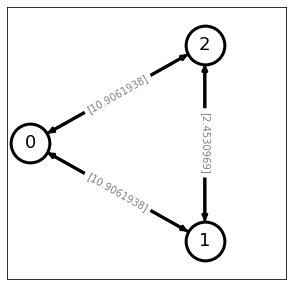
\includegraphics[scale=0.5]{img2.png}
\end{center}

We can see that there is significant difference in the demands between 2 to 0 and 0 to 1. Therefore it is better to satisfy the demand from 1 to 2 through this path, instead of opening a new channel.
By using the above method, we get that the requirements are sufficed by only 2 direct channels, in the following topology, and with total deposit of $\sim 44$/\\
\begin{center}
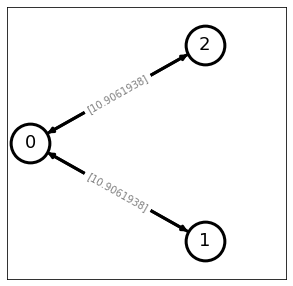
\includegraphics[scale=0.5]{img1.png}
\end{center}


\newpage
\section{Simulation Results}
We ran a simple simulation on our POC algorithm with the following configuration: 
\begin{enumerate}
    \item 10 different users ($N = 10$).
    \item Changing amount of off-chain payment demands ($d \in [1, 35]$).
    \item We compared our algorithm results to a naive deposit per-demand approach, where we are establishing a payment channel for each demand between 2 users.
\end{enumerate}

\\\\
In order to reach more conclusive results, we need to run tests that need more effort in terms of compute and time.\\\\

The results were encouraging as when the number of total demands increased the saving of our algorithm also increased. as seen in figure \ref{fig:results}

\begin{figure}[h]
\begin{subfigure}{0.5\textwidth}
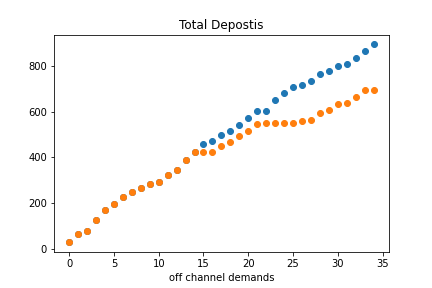
\includegraphics[width=1\linewidth, height=5cm]{exp10(1).png} 
\caption{Total deposits, our algorithm VS. naive approach}
\label{fig:total_deposits}
\end{subfigure}
\begin{subfigure}{0.5\textwidth}
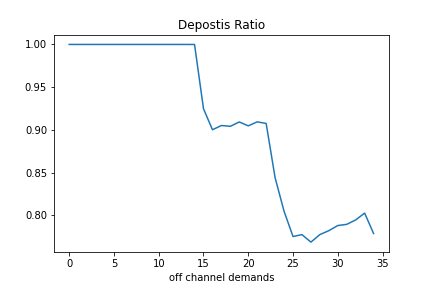
\includegraphics[width=1\linewidth, height=5cm]{exp11.png}
\caption{Deposits savings}
\label{fig:deposits_davings}
\end{subfigure}
\caption{Experiments results}
\label{fig:results}
\end{figure}

\\
in figure \ref{fig:total_deposits} We noticed that at the first iterations the total deposits are equal, while at a certain point, when there are enough channels that can be shared, the deposits in our algorithm grows slower.

\newpage
\section{Further Research}
There are several area where we think there is a possibility to further investigate this subject.
\begin{enumerate}
    \item Removing some of the simplicity assumptions in order to find better generic algorithm such as:
    \begin{itemize}
        \item The addition $A$ in each iteration of algorithm[2] must be a non-negative.
        \item The weights of the demands are equal: $w(c) = \frac{1}{N}$.
        \item The capacities on each channel are identical for both sides.
        \item Forcing each channel survivability to hold: $S(c)>=S_0$.
    \end{itemize}
    \item Collect data from real Transactions, in order to analyze the transactions distribution and model it accordingly to the algorithm (independent Gaussian variable between each 2 users). 
    \item Exploring other ways to model the payment demand between 2 users.
\end{enumerate}

\newpage
\section{Appendix}
\textbf{Understanding the intuition behind the usage of Gaussian distribution:}\\
Lets denote a channel $c$ between the users $u$ and $v$ on which there is only one demand: $d_{u,v} \sim \mathcal{N}(2, 0.5) $.\\
therefore, in order to hold a survivability of $S(c) = 0.9$ we need to add a capacity on the channel between $u$ and $v$ to hold the payments:\\
$C_u = 2.45$ and $C_v=0$ and the distribution is displayed in figure \ref{fig:dist1}.
\begin{figure}[h]
\caption{Gaussian distribution and the needed deposits on channel $c_{u,v}$}
\centering
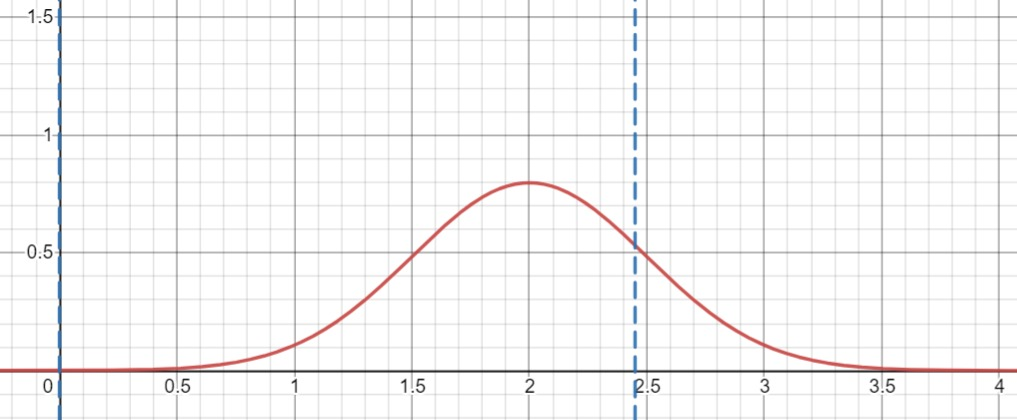
\includegraphics[scale=0.3]{Gauss_dist_1.jpeg}
\label{fig:dist1}
\end{figure}

Total capacity needed on this channel to satisfy the survivability condition is:
\begin{center}
    $C_{total} = C_u + C_v = 2.45$
\end{center}
\\
but, if there is another demand between users $x$ and $y$ where: $d_{x,y} \sim \mathcal{N}(2, 0.3)$ and we choose to route this demand over channel $c_{u,v}$ from the direction of $v$ to $u$. then the new distribution over the channel from direction $u$ to $v$ is: 
\begin{center}
 $\mathfrak{D}_{u,v}  \sim \matchcal{N}(2-2, 0.5+0.3) = \matchcal{N}(0, 0.8) $
\end{center}
\\
Therefore the new capacities needed on this channel are:
$C_u = 0.9$ and $C_v=0.9$ and the distribution is displayed in figure \ref{fig:dist2}.
\begin{figure}[h]
\caption{Gaussian distribution and the needed deposits on channel $c_{u,v}$}
\centering
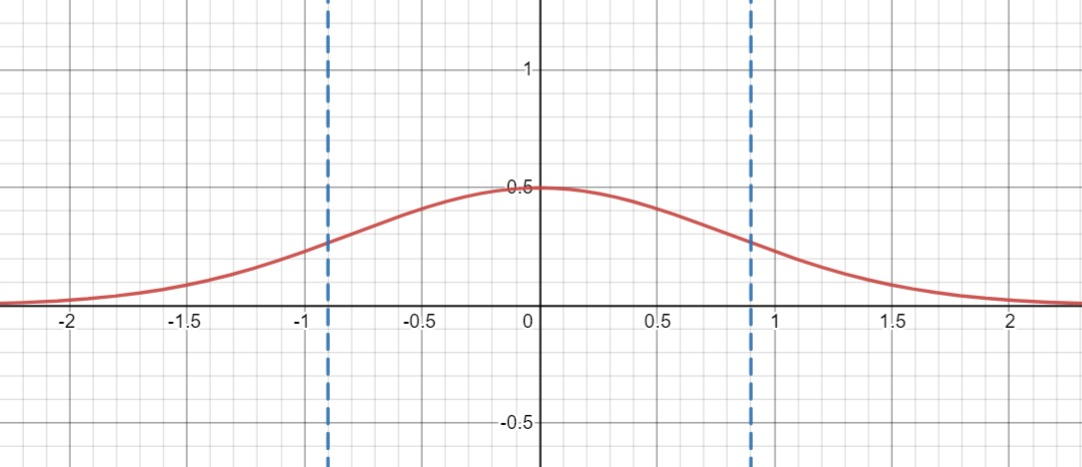
\includegraphics[scale=0.3]{Gauss_dist_2.jpeg}
\label{fig:dist2}
\end{figure}
\\
Total capacity needed on this channel to satisfy the survivability condition is:
\begin{center}
    $C_{total} = C_u + C_v = 1.8 < 2.45$
\end{center}
\\
In conclusion, sometimes, its better to equalize the mean value of the money transferred on the channel in order to lower the needed capacity to hold the Survivability conditions.\\
\\\\

\printbibliography



\end{document}
